\section{Introduction}
\label{sec:intro}

Recommendation systems is a primary example of the mainstream
applications of large scale data mining.  Applications such as online
adversiting, e-commerce website, personalized search, social network
and etc, make use of similar techniques to mine very sparse and large
scale data to better match users’ needs in a personalized fashion.
How to provide effective personalzied recomendation for large scale
and sparse data, becomes one of the most important research topics in
the past few decedes.


Online adverstising, one typical application of recommendation
systems, is a multi-billion dollar business which accounts for
majority of the revenue for companies like Google and Facebook. It is
a very complicated ecosystem, and involves multiple players, including
advertisers, publishers, end users and many others.  It allows
publishers in the network of content sites to serve automatic
advertisements (for text, image, videos, or interactive media), which
are targeted to site content and audience.
%
Take Google Adsense system ~\cite{adsense:wiki} as an example,
Figure~\ref{fig:adsense} illustrates how it works in a netshell: {\em
  Publisher} posts content on the Internet, and insert a code snippet
into its web pages. {\em User} visits the web page, which triggers the
code snippet to pull relevant advertisements from Google Adsense
servers, and show them on the same web page.  If user click on the
advertisement, the {\em advertiser} who created it will pay Google
certain amount of money, and Google will share majority of that
payment with the content publisher.
%
Google Adsense system generates billions of dollars each year,
supports hundreds of millions of publishers on the Internet
eco-system, and can reach more than 80\% of all Internet users
worldwide in more than 30 languages and over 100 countries.
%

\begin{figure}[!ht]
  \centering
  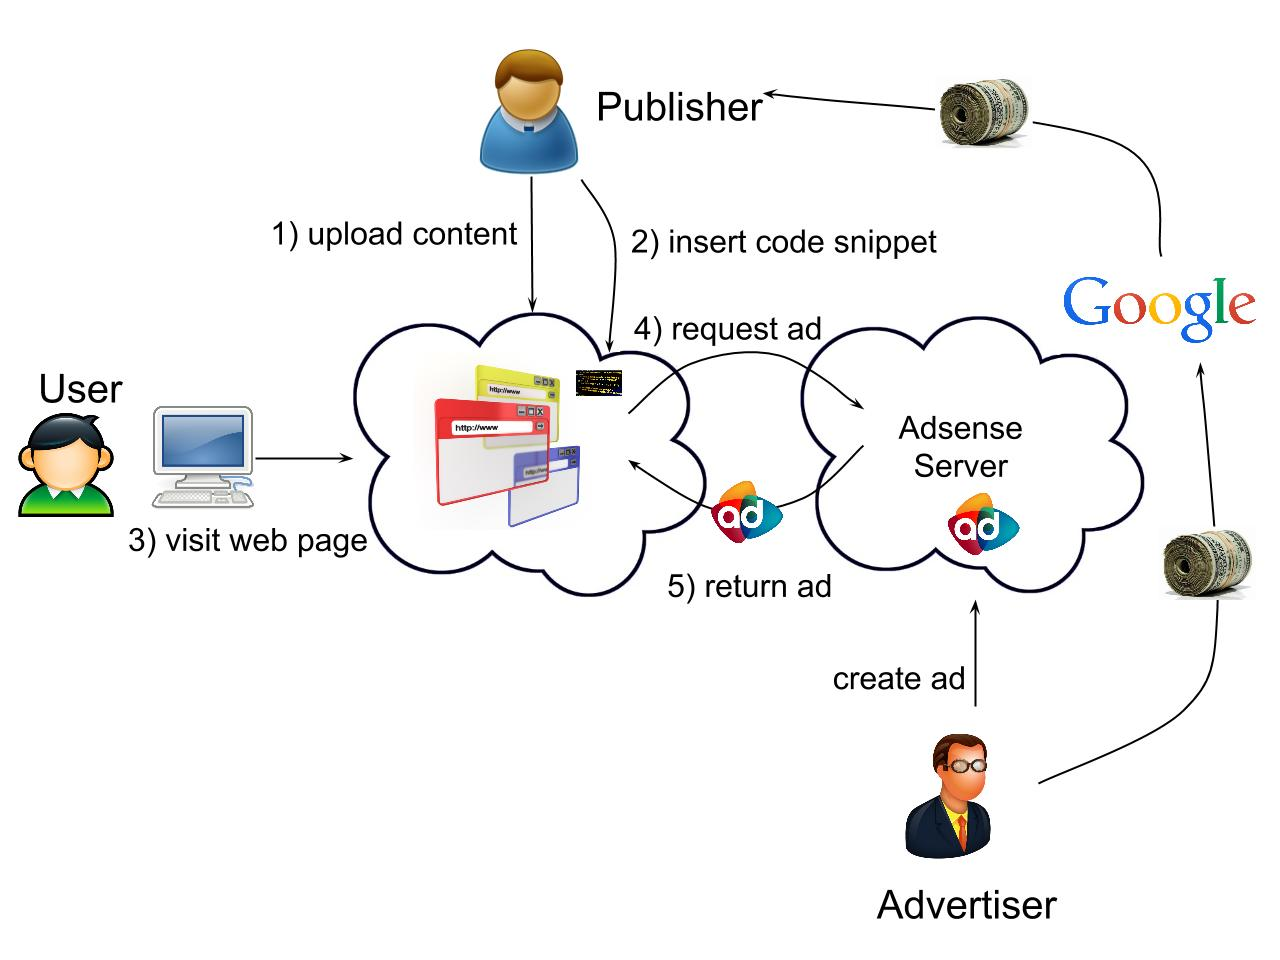
\includegraphics[width=0.4\textwidth]{figures/adsense.jpg}
  \caption{Google Adsense system work flow.}
  \label{fig:adsense}
\end{figure}

Delivering the right marketing messages to the right users in the
right time is of great importance to the success of online advertising
system. It requires the advertisers to provide a good list of
keywords, to match advertisements with web contents precisely, to
increase the click through rate and get a better advertisement
performance.
%
However, the reality is most advertisers are lack of experience to
provide good keywords for their advertisements. Therefore, how to make
best use of historical data to provide effective personalized keyword
recommendations is crutial to the success of Adsense. There are mainly
two types of approaches: A/B-testing and model based solutions.
 
A/B-testing~\cite{abtest:wiki} is widely used in online
advertisement. It splits the web traffice into two parts: majority of
the traffic uses the original keyword list to match advertisement, and
the other small fraction of the trafic uses the new keyword list,
which combine original keyword list along with some semantically
relevant keywords.  The experiments would be executed for some period
of time, usually in days or weeks, and then compare the statistics. If
the new list performs significantly better, we would surface this
recommendation to the advertiser.  The main drawback of this approach
is the long turnaround time. Lots of business opportunities may be
lost after days or weeks of experiments.

Model based solutions using collaborative
filtering~\cite{resnick1997recommender,sarwar2001item} comes into the
picture soon, which makes use of machine learning technology and
predicts the performance of the new keyword list without running
experiments. There are three type of collaborative filtering models
that are commonly used, user neighborhood model (considering the
similarity between users, in our case will be advertisers), item
neighborhood model (considering the similarity between items, in
oursecase will be keywords), and matrix factorization based
model~\cite{}. The matrix factorization based model has drawn a lot of
attention recently due to its success in the Netflix
Challenge~\cite{}. It's proven to produce better estimates than user
neighborhood or item neighborhood models, and can handle sparse data
set like the data in Netflix Challenge.
%
However, the data set we deal with is more than 100 times sparser than
the Netflix data. We observe significant overfitting even with very
strong regularization.

In this paper, we design a novel machine learning model that is
resilient to extremely sparse data set and doesn't need long
turnaround time in experiments.  First, the complexity of the model
(a.k.a. the number of parameters) grows with respect to observed data,
not to the number of advertisers and number of keywords like matrix
factorization based models. This makes our model resilient to
extremely sparse data. Secondly, our training algorithm is based on
gradient descent, which is easy to parallelize, and thus can handle
very large scale data set. Thirdly, our model combines the user
neighborhood and item neighborhood ideas in collaborative filtering
smartly, where similarities are ``learned'' from training algorithm
other than defining a global similarity metric for neighborhood.  All
these makes our model can efficiently handle extremely large scale
sparse data in an cost-effective way.

In summary, our main contributions in this paper include:
\begin{itemize} \itemsep -1pt
\item We successfully exploit the potential of improving personalized
  recommendation for extremely sparse and large scale data.
\item We develop a nodel model which uses gradient descent to combine
  user based and item based recommendation in a multi-dimension way,
  hence control the complexity with respect to observed data with
  short turnaround time.  We have implimented a distrubted training
  system that can handle large scale data set.
\item We apply our model successfully to personalized keyword
  recoomendation system in Google Adsense. The solution can be easily
  leveraged in all other online recommendation applications.
\item We conduct extensive comparison experiments with matrix
  factorization based methods and demonstrate that SPAN can
  effectively make personalized recommendation for extremly sparse and
  large scale data.
\end{itemize}

The remainder of this paper is organized as follows. We first
formulate the problem in Section~\ref{sec:problem}. Then we describe
the details of our model, including the high-level workflow, intuition
and assumptions, as well as different components of the model in
Section~\ref{sec:model}. After that, we introduce the training
algorithms in Section~\ref{sec:trainer}. We evaluate the effectiveness
and robustness of the proposed approach in Section~\ref{sec:exp}.  The
related works are reviewed in Section~\ref{sec:related}. Finally,
Section~\ref{sec:conclusion} concludes the paper and discusses future
directions of this study.
